\documentclass{scrartcl}
\usepackage{pgfplots}
\begin{document}

	\title{Compte-rendu de travaux pratiques de physique}
	\subtitle{Mesure de longueurs d'onde et célérités de phénomènes ondulatoires}
	\author{Benjamin Loison et Sara de Francqueville (MPSI 1)}
	\date{24 novembre 2018}
	\maketitle

	\section{Ondes ultrasonores}

	\subsection{Utilisation d'une mesure de déphasage}

	Aux travaux pratiques précédents, on a montré que si les deux signaux sont en phase alors en mode XY sur l'oscilloscope nous observons un segment de droite à pente strictement positive.
	
	On mesure la distance parcourue en déplaçant le récepteur mobile après 10 remises en phase afin de réduire l'erreur. Nous obtenons alors une distance de 9 centimètres, on en conclut que la longueur du signal est d'environ $\frac{10}{9}$ cm soit 1.11 cm.
	
	Ayant réglé la fréquence $\nu$ à 40 kilohertz, on a:
		$$\lambda=\frac{c}{\nu}$$
	Soit:
		$$c=\lambda*\nu$$
	D'où par application numérique:
		$$c=\frac{10}{9}*10^{-2}*40*10^3$$
	Donc:
		$$c=\frac{4000}{9}\ m.s^{-1}$$
	Soit:
		$$c=444.44\ m.s^{-1}$$
		
		Les mesures sont effectuées à la règle millimétrée donc on a une précision $\Delta$ = 0.5 mm soit 0.05 cm. On a alors l'incertitude sur la mesure de la des 10 remises en phase: $d$ = 9 $\pm$ 0.05 cm d'où: $\lambda$ = 1.11 $\pm$ 0.005 cm.\\
		% besoin incertitude sur le générateur

	\subsection{Interférences}
	
	  La distance $a$ mesure 5.4 centimètres. On prend $d$ = 60 cm.
		
		On relève les valeurs suivantes:
		
		\bigskip
		\begin{tabular}{|c|c|}
			\hline $\Delta x$ (en cm) & $\Delta V$ (en mV) \\
			\hline 0.0 & 7.6 \\
			\hline 0.5 & 11.0 \\
			\hline 1.0 & 12.4 \\
			\hline 1.5 & 14.6 \\
			\hline 2.0 & 15.6 \\
			\hline 2.5 & 16.8 \\
			\hline 3.0 & 17.0 \\
			\hline 3.5 & 18.6 \\
			\hline 4.0 & 20.0 \\
			\hline 4.5 & 19.2 \\
			\hline 5.0 & 18.6 \\
			\hline 5.5 & 16.8 \\
			\hline 6.0 & 13.4 \\
			\hline 6.5 & 13.0 \\
			\hline 7.0 & 10.8 \\
			\hline 7.5 & 9.4 \\
			\hline 8.0 & 5.8 \\
			\hline 8.5 & 3.6 \\
			\hline 9.0 & 5.6 \\
			\hline 9.5 & 8.0 \\
			\hline 10.0 & 9.6 \\
			\hline 10.5 & 10.0 \\
			\hline 11.0 & 12.2 \\
			\hline 11.5 & 13.8 \\
			\hline 12.0 & 14.6 \\
			\hline 12.5 & 14.6 \\
			\hline 13.0 & 14.6 \\
			\hline 13.5 & 16.2 \\
			\hline 14.0 & 15.2 \\
			\hline 14.5 & 15.0 \\
			\hline 15.0 & 13.8 \\
			\hline 15.5 & 12.2 \\
			\hline 16.0 & 11.4 \\
			\hline 16.5 & 9.6 \\
			\hline 17.0 & 8.6 \\
			\hline 17.5 & 6.8 \\
			\hline 18.0 & 6.4 \\
			\hline
		\end{tabular}

		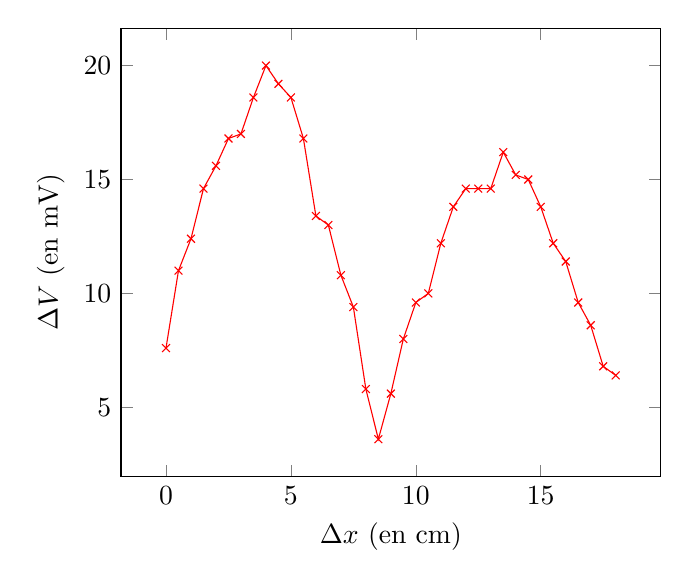
\begin{tikzpicture}
			\begin{axis}[
				xlabel=$\Delta x$ (en cm),
				ylabel=$\Delta V$ (en mV)]
			\addplot[color = red, mark = x] coordinates {
				(0.0,7.6)
				(0.5,11.0)
				(1.0,12.4)
				(1.5,14.6)
				(2.0,15.6)
				(2.5,16.8)
				(3.0,17.0)
				(3.5,18.6)
				(4.0,20.0)
				(4.5,19.2)
				(5.0,18.6)
				(5.5,16.8)
				(6.0,13.4)
				(6.5,13.0)
				(7.0,10.8)
				(7.5,9.4)
				(8.0,5.8)
				(8.5,3.6)
				(9.0,5.6)
				(9.5,8.0)
				(10.0,9.6)
				(10.5,10.0)
				(11.0,12.2)
				(11.5,13.8)
				(12.0,14.6)
				(12.5,14.6)
				(13.0,14.6)
				(13.5,16.2)
				(14.0,15.2)
				(14.5,15.0)
				(15.0,13.8)
				(15.5,12.2)
				(16.0,11.4)
				(16.5,9.6)
				(17.0,8.6)
				(17.5,6.8)
				(18.0,6.4)
			};
			\end{axis}
		\end{tikzpicture}
		
		On relève les deux maximums d'ordonnées pour les couples suivants: (4.0, 20.0) et (13.5, 16.2). Par différence des abscisses on obtient une interfrange $\Delta=9.5$ cm.
		
		On utilise la formule:
		$$\Delta=\frac{\lambda*d}{a}$$ avec $d$ la distance entre les émetteurs et le récepteur et $a$ la distance entre les deux émetteurs.
		D'où:
		$$\lambda=\frac{\Delta*a}{d}$$
		Par application numérique, on a:
		$$\lambda=\frac{9.5*10^{-2}*5.4*10^{-2}}{60*10^{-2}}$$
		Soit:
		$$\lambda=8.55*10^{-3}\ m$$
		Donc on obtient un résultat proche d'un centimètre comme nous l'avions mesuré.

	\section{Corde de Melde}
	
		On utilise la formule suivante afin de déterminer la longueur d'onde $\lambda$:
		$$\frac{L}{n}=\frac{\lambda}{2}$$ avec $L$ la longueur de la corde et $n$ le nombre de faisceaux observés.
		Soit:
		$$\lambda=\frac{2L}{n}$$
		Application numérique:
		$$\lambda=\frac{2*1.62}{2}=1.62\ m$$
		Puis on utilise la formule suivante afin de déterminer la célérité $c$ de l'onde parcourant la corde:
		$$\lambda=\frac{c}{\nu}$$ avec $\nu$ la fréquence de l'onde réglé nous-même sur le générateur basse-fréquence.
		Soit:
		$$c=\lambda*\nu$$
		Par application numérique, on a:
		$$c=1.62*35=57.75\ m.s^{-1}$$
		
		On détermine maintenant cette célérité à l'aide de la formule théorique. On calcule la tension $T$:
		$$T=mg$$ avec $m$ la masse du poids mis après la poulie et $g$ la constante de gravité terrestre.
		D'où par application numérique, on a:
		$$T=200*10^{-2}*10=2\ N$$
		On calcule la masse linéique $\mu$:
		$$\mu=\frac{m}{L}$$
		Par application numérique, on a:
		$$\mu=\frac{1.5}{1.62}$$
		Donc:
		$$\mu=0.93\ g.m^{-1}$$
		Soit:
		$$\mu=9.3*10^{-4}\ kg.m^{-1}$$
		
		On calcule alors la célérité théorique:
		$$c=\sqrt{\frac{T}{\mu}}$$
		D'où par application numérique, on a:
		$$c=\sqrt{\frac{2}{9.3*10^{-4}}}$$
		Donc:
		$$c=46.37\ m.s^{-1}$$
		Cette célérité théorique est proche de la célérité mesurée précédemment.
				
		\subsection{$c$ varie comme la racine carrée de $T$}
		
		On veut montrer que $c$ est proportionnelle à $\sqrt{T}$. Or $c$ = $\lambda * f$.\\
		On a:\\
		$[c]$ = $m/s$\\
		$[\lambda]$ = $m$\\
		$T$ = $m.g$\\
		$[f]$ = $Hz$\\
		On va chercher à obtenir 2 ventres pour différentes valeurs de $m$ en faisant varier la fréquence $f$ avec $\lambda$ = 138 cm.\\
		50 g $\rightarrow$ 21 Hz\\
		100 g $\rightarrow$ 29 Hz\\
		150 g $\rightarrow$ 36 Hz\\
		200 g $\rightarrow$ 42 Hz\\
		250 g $\rightarrow$ 46 Hz\\
		On peut à présent faire une régression linéaire avec $c$ en ordinnée et $\sqrt{T}$ en abscisse. On obtient une droite qui passe par l'origine. Conclusion c'est propotionnelle à $\sqrt{T}$.
				
		\subsection{la fréquence de résonance $f_n$ du n-ième mode propre est inversement proportionnelle à la longueur $L$ de la corde}

		On veut montrer que $f_n$ est proportionnel à $\frac{1}{L}$
		On fait donc la même chose en faisant varier $L$ la longueur de la corde, pour 2 ventres donc en fonction de la fréquence $f$ nécessaire.\\
		On obtient une droite qui passe par l'origine en fesant une régression linéaire. Donc $L$ est inversement proportionnelle à $f_n$.\\\\
		
		On a la relation: $c$ = $\sqrt{\frac{T}{\mu}}$ avec $\mu$ = $m_corde$ * $L_corde$. On a ici: $T$ = $100 * 10^{-3} * 9.81 m^2.s^{-2}$ et $\mu$ = $0.9 * 10^{-3}*138 * 10^{-2} kg.m.$.\\
		Donc $c$ = $\sqrt{\frac{100 * 10^{-3} * 9.81}{0.9 * 10^{-3}*138 * 10^{-2}}}$ = $2.81 m/s$. On sait que $\lambda$ = $\frac{2L}{n}$ avec $n$ le nombre de ventres. Donc dans notre situation $c'$ = $\frac{2*138*10^{-2}}{2}*29$ = 40.0. Onremarque un léger écart entre les deux valeurs. On écrit l'écart relatif: $\frac{|c-c'|}{c}$ = $\frac{|28.1-40.0|}{28.1}$ = 0.42. Soit 42 \%. Ceci est non négligeable.  

\end{document}